\documentclass[aps,prb,onecolumn,notitlepage,showpacs,floatfix,superscriptaddress]{revtex4-1}
\usepackage{dcolumn}
\usepackage{tabularx}
\usepackage{bm}
\usepackage{soul}
\usepackage{amsmath,xcolor}
\fboxrule=1pt
\usepackage{amssymb,graphicx}
\usepackage[colorlinks=true,citecolor=blue,urlcolor=blue,linkcolor=blue]{hyperref}
\usepackage{environ}

\usepackage{tikz}
\usetikzlibrary{matrix}
\usetikzlibrary{fit}

\NewEnviron{eqnsplit}{%
\begin{equation}
\begin{split}
  \BODY
\end{split}
\end{equation}
}
\newcommand{\mrm}[1]{\mathrm{#1}}
\newcommand{\AR}[1]{\textcolor{red}{#1}}
\newcommand{\ang}{\mathrm{\AA}}

\bibliographystyle{apsrev4-1}

%%%%%%%%%%%%%%%%%%%%%%%%%%%%%%%%%%%%%%%%%%%%%%%%
\begin{document}
\title{EPR Paradox and Bell's Inequality}

\author{Avinash Rustagi}
\email{arustag@purdue.edu}
%
%\date{\today}
%%%%%%%%%%%%%%%%%%%%%%%%%%%%%%%%%%%%%%%%%%%%%%%%

\maketitle
%
%\noindent \textcolor{blue}{Reference: Phys. Rev. Lett. 30, 230 (1973)}
%\vspace{0.2in}

\section{EPR Paradox}
Einstein - Podolsky - Rosen (EPR) paradox is a thought experiment that was proposed to argue that the physical description of nature as described by quantum mechanics was incomplete. What this means that the three physicists believed that there was more to quantum mechanics i.e. \textit{hidden variables} that determined the outcomes of experiments. The use of probability when it came to statistical mechanics was mainly due the fact that there was incomplete information known about the system when it came to a large number of degrees of freedom. However, what they did not accept was that quantum mechanics if complete should not be probabilistic. Thus, came forward the `hidden variable theory'.\\

\begin{center}
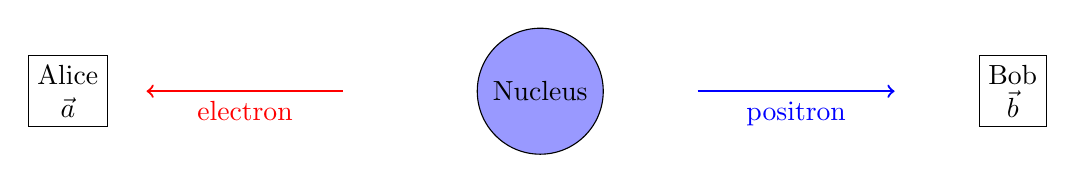
\begin{tikzpicture}
\node[draw,align=center] at (-1,0) {Alice \\ $\vec{a}$ };
\draw[red,thick,<-] (0,0) -- (2.5,0) node[midway,below] {electron} ;
\filldraw[fill=blue!40!white, draw=black] (5,0) circle (0.8cm) node[label=center:Nucleus]{}; 
\draw[blue,thick,->] (7,0) -- (9.5,0) node[midway,below] {positron} ; 
\node[draw,align=center] at (11,0) {Bob \\ $\vec{b}$ };
\end{tikzpicture}
\end{center}

For the thought experiment, let us imagine that we have two observers Alice and Bob who are spatially separated by a long distance. Midway between them is an unstable nucleus that decays emitting an electron that propagates towards Alice and a positron that propagates towards Bob. What everyone can agree on is the conservation of angular momentum before and after the decay. What this implies that the spins of the electron and positron if measured along the same quantization axis will be opposite. Let us assume that Alice makes a measurement on the spin of the electron first along the quantization axis of her choice namely $\vec{a}$ and measures +1/2. Now, if Bob were to measure the spin of the positron along the same quantization axis i.e. $\vec{a}$, then he will find the spin to be -1/2. This implies that there exists correlation between the measurements.\\

Let us now consider the predictions of quantum mechanics of these measurements. Without loss of generality, we can choose z-axis to be along $\vec{a}$ (the direction along which Alice measures the spin). Thus, before Alice measures, the quantum mechanical state of the electron-positron system can be written as
\begin{equation}
\vert \Psi \rangle = \dfrac{1}{\sqrt{2}} \left[ \vert e, \uparrow_{\vec{z}} \rangle \vert p, \downarrow_{\vec{z}} \rangle - \vert e, \downarrow_{\vec{z}} \rangle \vert p, \uparrow_{\vec{z}} \rangle  \right] 
\end{equation}
After Alice measures the electron's spin and finds it to be +1/2, the state of the system collapses to 
\begin{equation}
\vert \Psi \rangle = \vert e, \uparrow_{\vec{z}} \rangle \vert p, \downarrow_{\vec{z}} \rangle
\end{equation}
At this point, Bob is free to make a choice on the spin measurement axis and say he chooses to measure the spin of positron along $\vec{b}$ at an angle $(\theta,\phi)$ wrt the z-axis. The spin state with quantum number +1/2 along $\vec{b}$ can be related to the spin state along $\vec{z}$ (which is nothing but the change of basis),
\begin{equation}
\vert p, \uparrow_{\vec{b}} \rangle = \cos\dfrac{\theta}{2} e^{-i\phi/2} \vert p, \uparrow_{\vec{z}} \rangle + \sin\dfrac{\theta}{2} e^{i\phi/2} \vert p, \downarrow_{\vec{z}} \rangle
\end{equation}
Thus, the probability that Bob measures +1/2 along $\vec{b}$ can be evaluated by the Born rule
\begin{equation}
\begin{split}
P(\vec{b},+1/2) &= \vert \langle p, \uparrow_{\vec{b}} \vert p, \downarrow_{\vec{z}} \rangle \vert^2 = \sin^2 \dfrac{\theta}{2} \\
P(\vec{b},-1/2) &= \vert \langle p, \downarrow_{\vec{b}} \vert p, \downarrow_{\vec{z}} \rangle \vert^2 = \cos^2 \dfrac{\theta}{2} \\
\end{split}
\end{equation}
So far we have made no restrictions on the speeds with which the electron and positron moves. So let us now consider that they move at relativistic speeds and Alice and Bob make their measurement in the rest frame of the electron and positron. Now if we consider that Alice and Bob make the measurements simultaneously, then there is no way that a signal could have traveled from Alice's measurement on electron to Bob. So the paradox is that if there is no transfer of information, how is it possible that Bob's measurement depends on the outcome of Alice's measurement. \\


This led the EPR team to conclude that the information relating to the outcomes of the measurements must be pre-ordained in the state of the electron and positron. The variable in which this information is pre-ordained were referred to as Hidden Variables.

\section{Bell's Inequality}
John Bell derived an inequality that would test if quantum mechanics is consistent with the hidden variables theory or not. \\

\subsection{Quantum Mechanical Prediction}
To derive this inequality, let us label the measurement of the spin of the electron made by Alice along $\vec{a}$ as $\sigma_e (\vec{a})$ which can be $\pm$1/2. Similarly, the measurement of the spin of the positron made by Bob along $\vec{b}$ as $\sigma_p (\vec{b})$ which can be $\pm$1/2. Let us look at the expectation value of $\sigma_e \sigma_p$ given that Bob measures the spin of the positron soon after Alice measures the spin of electron,
\begin{equation}
\begin{split}
\langle \sigma_e(\vec{a}) \sigma_p(\vec{b}) \rangle &= \dfrac{1}{4} \bigg[ P\left(\vec{a},+\dfrac{1}{2}\right) P\left(\vec{b},+\dfrac{1}{2} \bigg\vert \vec{a},+\dfrac{1}{2}\right) +  P\left(\vec{a},-\dfrac{1}{2}\right) P\left(\vec{b},-\dfrac{1}{2} \bigg\vert \vec{a},-\dfrac{1}{2}\right) \\
&- P\left(\vec{a},+\dfrac{1}{2}\right) P\left(\vec{b},-\dfrac{1}{2} \bigg\vert \vec{a},+\dfrac{1}{2}\right) - P\left(\vec{a},-\dfrac{1}{2}\right) P\left(\vec{b},+\dfrac{1}{2} \bigg\vert \vec{a},-\dfrac{1}{2}\right) \bigg]
\end{split}
\end{equation}
where $P(\vec{a},\pm 1/2)$ is the probability for Alice to measure $\pm 1/2$ and $P(\vec{b},\alpha \vert \vec{a},\beta)$ is the conditional probability for Bob to measure the spin of positron to be $\alpha$ given that Alice measures the spin of electron to be $\beta$.\\


From quantum mechanics, we know that 
\begin{equation}
\begin{split}
P\left(\vec{a},\pm \dfrac{1}{2}\right) &= \dfrac{1}{2} \\
P\left(\vec{b},+\dfrac{1}{2} \bigg\vert \vec{a},+\dfrac{1}{2}\right) &= \sin^2\dfrac{\theta}{2} = P\left(\vec{b},-\dfrac{1}{2} \bigg\vert \vec{a},-\dfrac{1}{2}\right) \\
P\left(\vec{b},+\dfrac{1}{2} \bigg\vert \vec{a},-\dfrac{1}{2}\right) &= \cos^2\dfrac{\theta}{2} = P\left(\vec{b},-\dfrac{1}{2} \bigg\vert \vec{a},+\dfrac{1}{2}\right)
\end{split}
\end{equation}
which implies that quantum predicts 
\begin{equation}
\langle \sigma_e(\vec{a}) \sigma_p(\vec{b}) \rangle = -\dfrac{1}{4} \cos\theta = -\dfrac{1}{4} \vec{a} \cdot \vec{b}
\end{equation}

\subsection{Hidden Variable Theory Prediction}
The hidden variable theory is based on a set of variables $\vec{v}$ that define the outcome of the measurements such that
\begin{equation}
\sigma_e(\vec{v},\vec{a}) = \pm \dfrac{1}{2} \qquad \sigma_p(\vec{v},\vec{b}) = \pm \dfrac{1}{2} 
\end{equation}
and the conservation of angular momentum requires that if the measurement axis for Alice and Bob are the same, then
\begin{equation}
\sigma_e(\vec{v},\vec{a}) = - \sigma_p(\vec{v},\vec{a})
\end{equation}
Thus, as per the hidden variable theory, any measurement or expectation value needs to be averaged over the hidden variables via a probability distribution function $\rho(\vec{v})$, such that
\begin{equation}
\begin{split}
\langle \sigma_e(\vec{a}) \sigma_p(\vec{b}) \rangle_{\vec{v}} &= \int d\vec{v} \, \rho(\vec{v}) \sigma_e(\vec{v},\vec{a}) \sigma_p(\vec{v},\vec{b}) \\
&= -\int d\vec{v} \, \rho(\vec{v}) \sigma_e(\vec{v},\vec{a}) \sigma_e(\vec{v},\vec{b}) \\
\end{split}
\end{equation}
Let us now consider 
\begin{equation}
\begin{split}
\langle \sigma_e(\vec{a}) \sigma_p(\vec{b}) \rangle_{\vec{v}}-\langle \sigma_e(\vec{a}) \sigma_p(\vec{c}) \rangle_{\vec{v}} &=  -\int d\vec{v} \, \rho(\vec{v}) \sigma_e(\vec{v},\vec{a}) \left[ \sigma_e(\vec{v},\vec{b})-\sigma_e(\vec{v},\vec{c})\right] \\
&=  -\int d\vec{v} \, \rho(\vec{v}) \sigma_e(\vec{v},\vec{a}) \, 4 \sigma_e^2(\vec{v},\vec{b}) \left[ \sigma_e(\vec{v},\vec{b})-\sigma_e(\vec{v},\vec{c})\right] \\
&=  -\int d\vec{v} \, \rho(\vec{v}) \sigma_e(\vec{v},\vec{a}) \, \sigma_e(\vec{v},\vec{b}) \left[1-4\sigma_e(\vec{v},\vec{b}) \sigma_e(\vec{v},\vec{c})\right] \\
\end{split}
\end{equation}
Here, we have used the fact that $\sigma_e^2(\vec{v},\vec{a})=1/4$. We note that the terms in the square brackets is positive definite since the product $\sigma_e(\vec{v},\vec{b}) \sigma_e(\vec{v},\vec{c})$ can only take values $\pm 1/4$. Thus, $1-4\sigma_e(\vec{v},\vec{b}) \sigma_e(\vec{v},\vec{c}) \geq 0$. Given this, we can look at the absolute value of the left hand side (LHS) and utilizing the identity that $\vert \int d\vec{v} \, f(\vec{v}) \vert \leq \int d\vec{v} \, \vert f(\vec{v}) \vert $, we find that
\begin{equation}
\begin{split}
\vert \langle \sigma_e(\vec{a}) \sigma_p(\vec{b}) \rangle_{\vec{v}}-\langle \sigma_e(\vec{a}) \sigma_p(\vec{c}) \rangle_{\vec{v}} \vert  &\leq \int d\vec{v} \, \rho(\vec{v}) \dfrac{1}{4} \left[1-4\sigma_e(\vec{v},\vec{b}) \sigma_e(\vec{v},\vec{c})\right] \\
\end{split}
\end{equation}
where we have used the fact that $\vert \sigma_e(\vec{v},\vec{a}) \vert = \vert \sigma_e(\vec{v},\vec{b}) \vert = 1/2 $. Thus,
\begin{equation}
\begin{split}
\vert \langle \sigma_e(\vec{a}) \sigma_p(\vec{b}) \rangle_{\vec{v}}-\langle \sigma_e(\vec{a}) \sigma_p(\vec{c}) \rangle_{\vec{v}} \vert  &\leq \dfrac{1}{4}  \left[ 1 - 4 \int d\vec{v} \, \rho(\vec{v}) \sigma_e(\vec{v},\vec{b}) \sigma_e(\vec{v},\vec{c})\right] \\
&\leq \dfrac{1}{4}  \left[ 1 - 4 \langle \sigma_e(\vec{v},\vec{b}) \sigma_e(\vec{v},\vec{c})\rangle_{\vec{v}} \right] \\
&\leq \dfrac{1}{4}  \left[ 1 + 4 \langle \sigma_e(\vec{v},\vec{b}) \sigma_p(\vec{v},\vec{c})\rangle_{\vec{v}} \right] \\
\end{split}
\end{equation}
This is referred to as Bell's inequality. \\

\begin{figure}[hbtp]
\centering
\includegraphics[width=0.5\textwidth]{Figure_1.png}
\caption{Left and right hand side of Bell's inequality.}
\end{figure}

The question we address next is: Is quantum mechanics consistent with Bell's inequality?\\

From quantum mechanics, $\langle \sigma_e(\vec{v},\vec{a}) \sigma_p(\vec{v},\vec{b})\rangle = -\dfrac{1}{4} \vec{a} \cdot \vec{b}$. Thus, we can evaluate the LHS and RHS of the inequality using this
\begin{equation}
\text{LHS} = \dfrac{1}{4} \vert \vec{a} \cdot (\vec{b}-\vec{c}) \vert \qquad \qquad  \text{RHS} = \dfrac{1}{4} [1-\vec{b}\cdot \vec{c}]   
\end{equation}
If quantum mechanics is consistent with the hidden variable theory, then Bell's inequality must be satisfied irrespective of the choice of $\vec{a}$, $\vec{b}$, and $\vec{c}$. Let us choose $\vec{a}\cdot\vec{b} = 0$ and $\vec{c} = \sin\psi \, \vec{a} + \cos\psi \, \vec{b}$ where $\vec{a}$ is orthogonal to $\vec{b}$ and $\psi$ is the angle between $\vec{c}$ and $\vec{b}$. With this choice,
\begin{equation}
\text{LHS} = \dfrac{1}{4}\vert \sin\psi \vert \qquad \qquad  \text{RHS} = \dfrac{1}{4} [1-\cos\psi]   
\end{equation}
From this we can see that LHS $\geq$ RHS for all $\psi$ within the range from 0 to $\pi/2$ which contradicts Bell's inequality. \\

Thus, we can conclude that quantum mechanics is inconsistent with the hidden variable theory.
\end{document}
